\pagestyle{fancy}

\graphicspath{ {Figures/Chapter5_SimulationBenchmarking/} }


\section{LINAC4 Signal Generation Studies.}

As was introduced in \ref{sec:LINAC4}, LINAC4 accelerates \hm particles up to 160 MeV. \hm ions consist of one proton ($N_p$ = 1) and two electrons ($N_e$ = 2). In this case formula \ref{eq:Qsum} can be written as: 

\begin{equation}
    Q\left(\frac{e}{H^{-}}\right) = \eta - 2\mu + \left( 2 - \eta + BS_p \right) \cdot SEY_p +2\left( 2 - \mu - BS_e \right) \cdot SEY_e
    \label{eq:Ql4}
\end{equation}

Note that in this case, we are considering the secondary emission yield for electrons and protons to be the same at the entrance and the exit of the detectors. As we will see in the following, this might not be the most accurate procedure for some of the detectors at LINAC4. Figure \ref{fig:RangeLinac4} shows how the values of the range of protons change as a function of the particle energy. 

\begin{figure}[h]
    \centering
    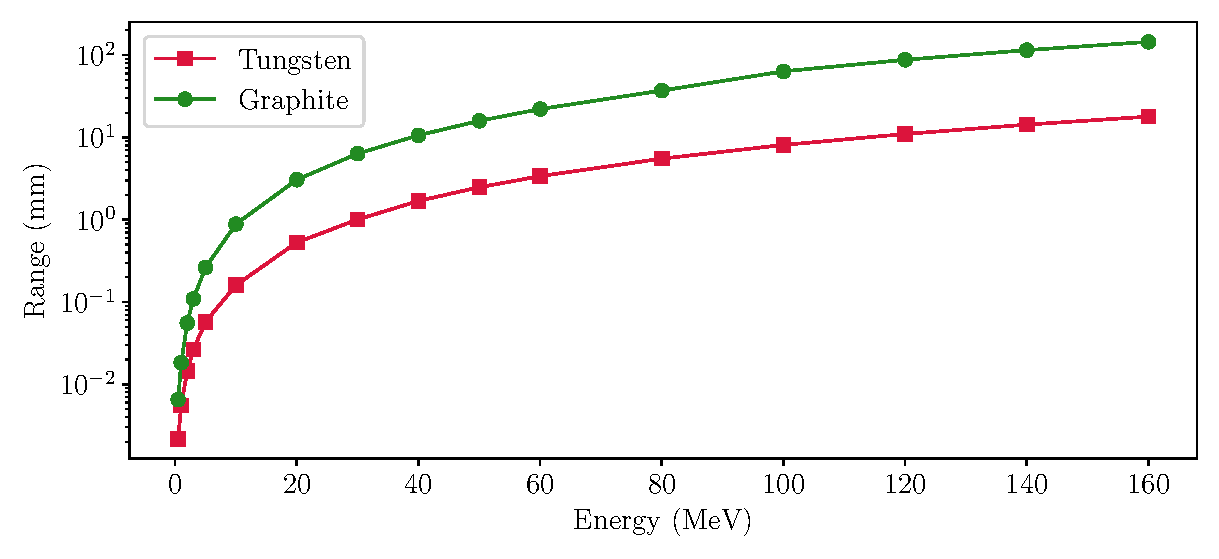
\includegraphics[width=0.9\columnwidth]{RangePlotLinac4/RangeL4.pdf}
    \caption{Range of particles as a function of incident ion energy.}
    \label{fig:RangeLinac4}
\end{figure}

From this figure, we can see how the range of the particles in the material increases as their energy increases. For the same energies, the particles have a much larger range in the case of graphite compared to tungsten. At LINAC4, the wires have a width of $40$ \si{\micro\metre} for the case of tungsten and 33 \si{\micro \metre} for the case of graphite wires. 

The range of protons is larger than the detector thickness in most of the energy range. Only tungsten detectors placed at energies smaller than 5  \si[]{\mega\electronvolt} are expected to get a positive charge deposition. The electrons in an \hm ion have energy much smaller than the proton. It is actually reduced a factor $m_p / m_e = 1836.15$ compared to the energy of the \hm ions.  Electrons are expected to deposit all their energy in all the SEM grids and Wire scanners at Linac4. So we expect to always have a double negative charge contribution. 

Table \ref{tab:ChargePar} summarizes the values for $\eta$ and $\mu$ parameters along the Linac4 accelerator range. This table also summarizes the values of the Backscattering probabilities for both electrons and protons. All these values have been calculated with Geant4 \parencite[][]{ref:Geant4}. The backscattering probability is negligible for the protons. Contrarily, electron backscattering probability is not negligible. In the case of tungsten, for ion energies of 160 MeV half of the electrons are backscattered.

% Please add the following required packages to your document preamble:
% \usepackage{multirow}
\begin{table}[h]
    \begin{tabular}{cccccccccc}
    \hline
    \multirow{2}{*}{\begin{tabular}[c]{@{}c@{}}$p^+$ energy \\ (MeV)\end{tabular}} & \multirow{2}{*}{\begin{tabular}[c]{@{}c@{}}$e^-$ energy\\ (keV)\end{tabular}} & \multicolumn{4}{c}{Graphite} & \multicolumn{4}{c}{Tungsten} \\ \cline{3-10}  &   & $\eta$   & $\mu$     & $BS_p$ & $BS_e$   & $\eta$ & $\mu$     & $BS_p$ & $BS_e$     \\ \hline
    3                                                                     & 1.63                                                                           & 0.001 & 0.918 & 0.0 & 0.081 & 1.0 & 0.632  & 0.0 & 0.367   \\
    50                                                                    & 27.23                                                                          & 0.0   & 0.931  & 0.0 & 0.068 & 0.0 & 0.506  & 0.0 & 0.493  \\
    102                                                                   & 55.55                                                                          & 0.0   & 0.887  & 0.0 & 0.112 & 0.0 & 0.487 & 0.0 & 0.512 \\
    160                                                                   & 87.14                                                                          & 0.0   & 0.857  & 0.0 & 0.142 & 0.0 & 0.464  & 0.0 & 0.536   \\ \hline
    \end{tabular}
    
    \caption{Summary of charge deposition and backscattering probabilities for Tungsten ($40 \mu m$) and Graphite ($33 \mu m$)} detectors.
    \label{tab:ChargePar}
\end{table}

Figure \ref{fig:SEYmat} shows the Secondary Emission yield calculated with the semiempirical Sternglass formula (Eq. \ref{eq:sey}) as a function of the incident proton energy.  In both materials, the SEY reaches a maximum ( $~ 0.1 $ MeV ) which is followed by a decrease in the SEY. Graphite presents a higher SEY at smaller proton energies whereas tungsten presents a higher SEY at higher incident particle eneriges. 

\begin{figure}[h]
    \centering
    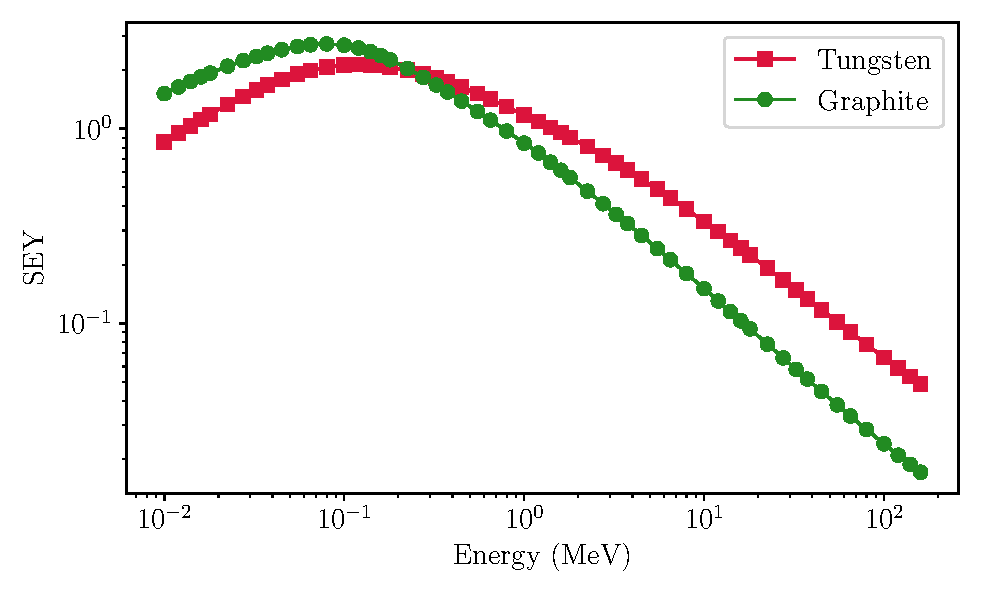
\includegraphics[width=0.85\columnwidth]{Figure_SEY/SEY_compa.pdf}
    \caption{Secondary Emission Yield as a function of incident proton energy. }
    \label{fig:SEYmat}
\end{figure}

As an example, figure \ref{fig:ProfComparison} shows a simulated beam profile at 3 MeV and 160 MeV. From these figures, we can observe how at 3 (MeV) the positive contribution to the charge is predominant for the case of tungsten wires while it remains negative in the case of graphite wires. Due to the smaller SEY of graphite at 160 (MeV), the absolute registered signal at this energy is higher than the one registered by the tungsten wires. 

\begin{figure}[h]
    \centering
    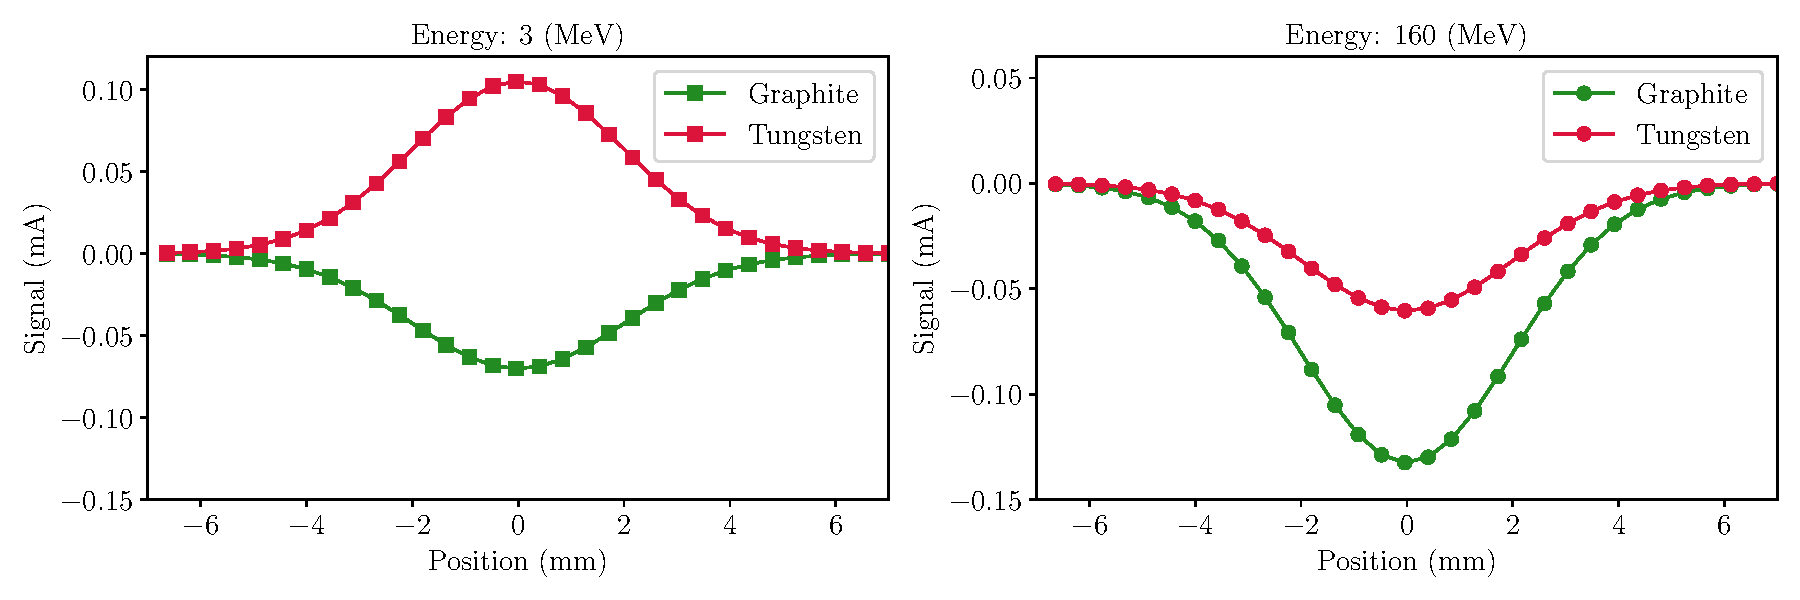
\includegraphics[width=0.85\columnwidth]{Figure_ProfCompa/ProfileComparison.pdf}
    \caption{Expected transverse beam profile for incident \hm particles. Left: 3 (MeV), Right: 160 (MeV). For these simulations, a 25 mA, 100 $\mu s$ particle beam was considered. }
    \label{fig:ProfComparison}
\end{figure}

At Linac4, even if these detectors are called Secondary Emission Monitors, the biggest contribution to the charge formation is the charge deposition term. To prevent misinterpretations, SE is typically suppressed by a bias current.  At LINAC4, the detectors at lower energies are usually conformed with graphite wires, to avoid the positive contribution of the proton charge deposition. 

\section{Beam Intensity and Profile Measurements at CERN LINAC4.}

In this section, we will briefly show how the instruments just presented are used at CERN, LINAC4. All the results presented in this section correspond to the first profile and current measurements for the LBE run, which took place in November 2019 \parencite*[][]{ref:PresentationLBERun}. The objective of these measurements was to study the transverse profile evolution of the particle beam along the LINAC4 accelerator. 

Figure \ref{fig:Linac4Layout} shows a schematic representation of LINAC4 with the different detectors and locations. In this figure, the yellow circles represent the BCTs. The blue and red rectangles indicate the positions of SEM grids and Wire scanners respectively. Green rectangles indicate positions where SEM grid and Wire scanners are installed at the same position. As we can see from this figure, both BCTs and Beam profile instruments are placed all along LINAC4 so the beam parameters can be measured in all the acceleration stages. 

\begin{figure}[h]
    \centering
    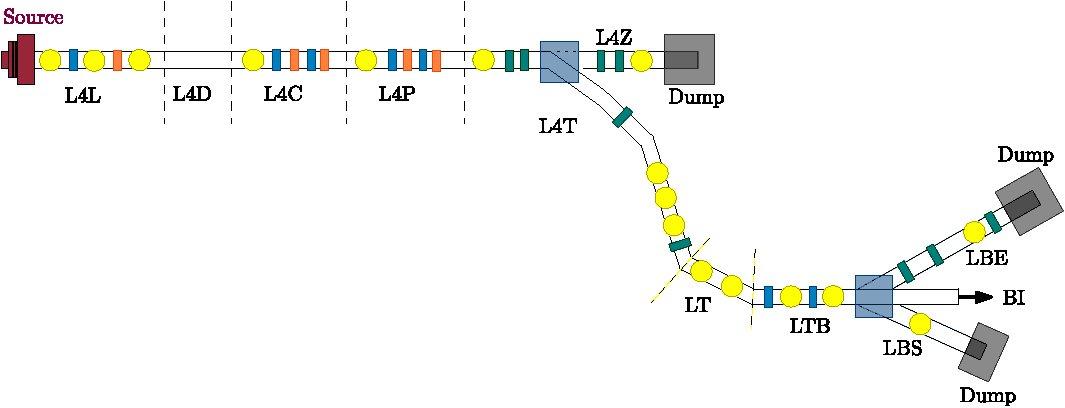
\includegraphics[width=1.0\columnwidth]{Linac4Instrumetnation/Linac4Instruments.pdf}
    \caption{Schematic representation of LINAC4 with the location of some diagnostics devices.}
    \label{fig:Linac4Layout}
\end{figure}

Figure \ref{fig:BCTwithTime} shows an example of intensity measurement taken by the first BCT in the L4T segment. From this figure, one can identify the beam pulse, we can observe that due to the accelerator of $H^{-}$ particles at LINAC4, the registered current is negative. In this case, the beam pulse length was 36 \si[]{\micro \second} with an average intensity of $\sim 17 $ \si[]{\milli \ampere}. One can observe the 1 \si[]{\micro \second} gaps generated by the chopper, which make the beam pulse ready to be injected into the different pulse rings. 

\begin{figure}
    \centering
    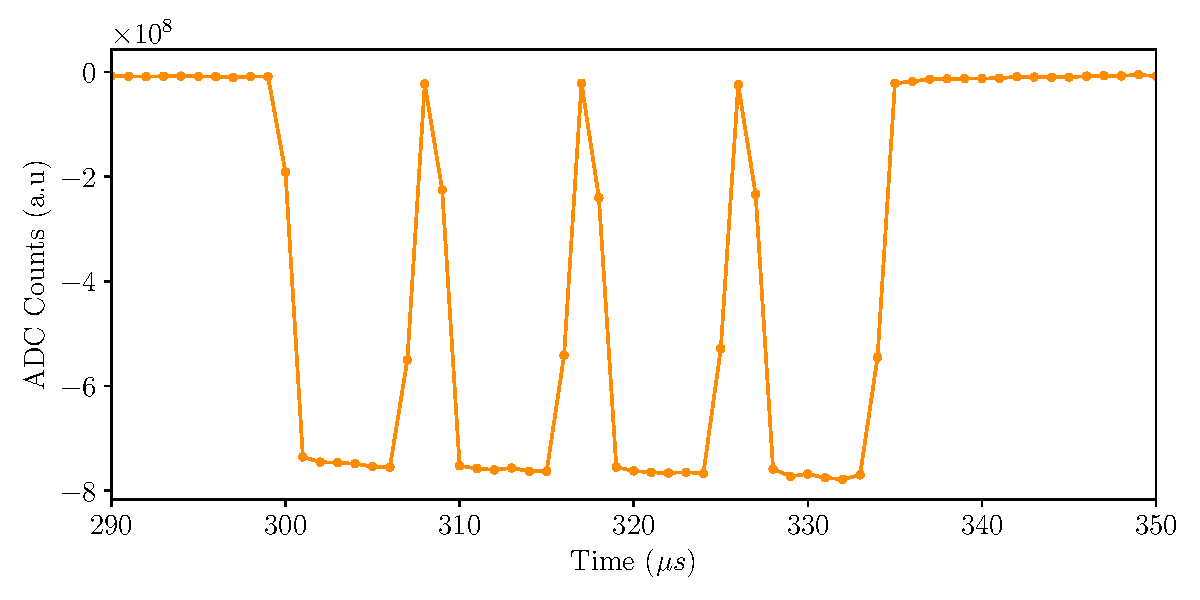
\includegraphics[width=0.7\columnwidth]{IntensityVStime/IntensityVStime.pdf}
    \caption[The LOF caption]{Beam current shape along beam pulse, from first BCT in L4T line.}
    \label{fig:BCTwithTime}
\end{figure}

By measuring the average current of the beam at all the available BCTs, one can assess the beam transmission along the accelerator. Figure \ref{fig:BeamTrans} shows an example of beam transmission measured along the accelerator. From this figure one can observe how in all parts of the accelerator, except for the first two BCTs in the L4L line, the current remains quite constant around $\sim 17$ \si[]{\milli \ampere}.  Similarly, the beam transmission remains very close to $100 \%$ along the whole accelerator. 

\begin{figure}
    \centering
    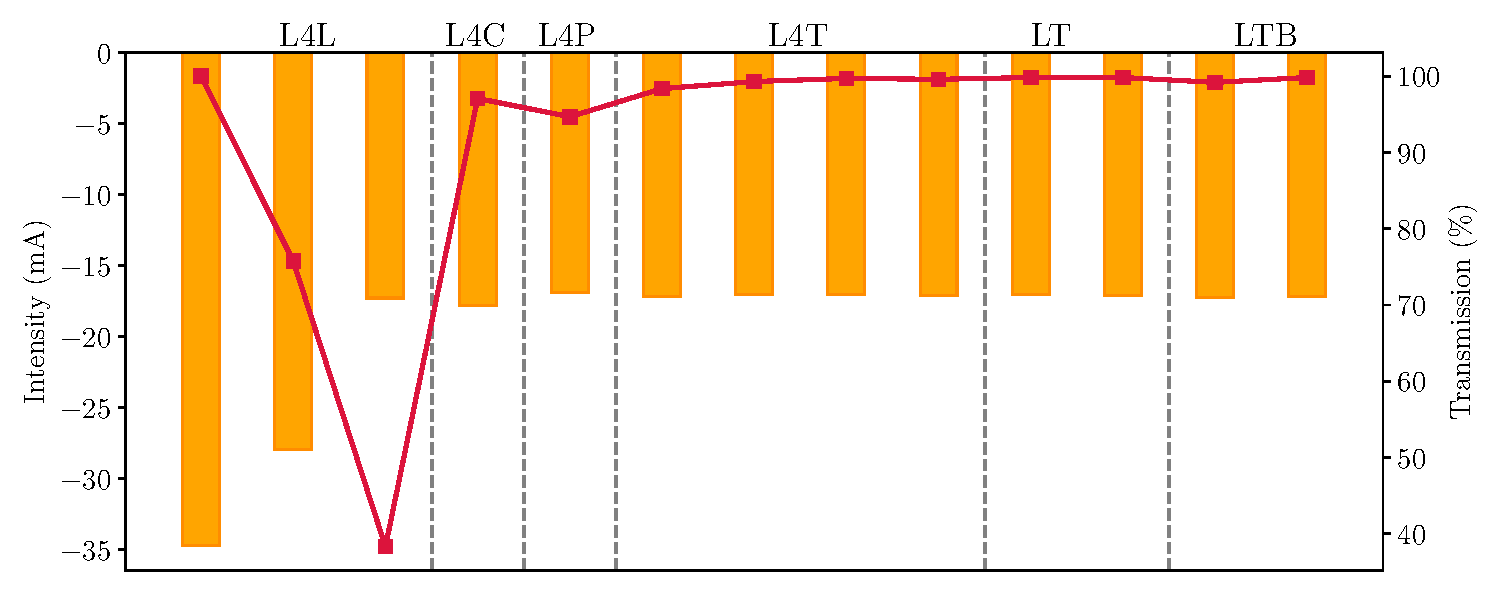
\includegraphics[width=0.9\columnwidth]{BCT_Transmission/TransmissionBCT.pdf}
    \caption{Average intensity measured by the different BCTs at LINAC4. Transmission along the LBE line.}
    \label{fig:BeamTrans}
\end{figure}

Similarly, the beam profile was measured along the accelerator, to cross-check the beam evolution as well as to assess the integrity and status of the devices installed along the accelerator.  Figure \ref{fig:HorizontalProf} shows the measurements of the horizontal profile of the beam along the LINAC4 accelerator. All these measurements were taken with the SEM grids. From this figure we can observe:

\begin{figure}
    \centering
    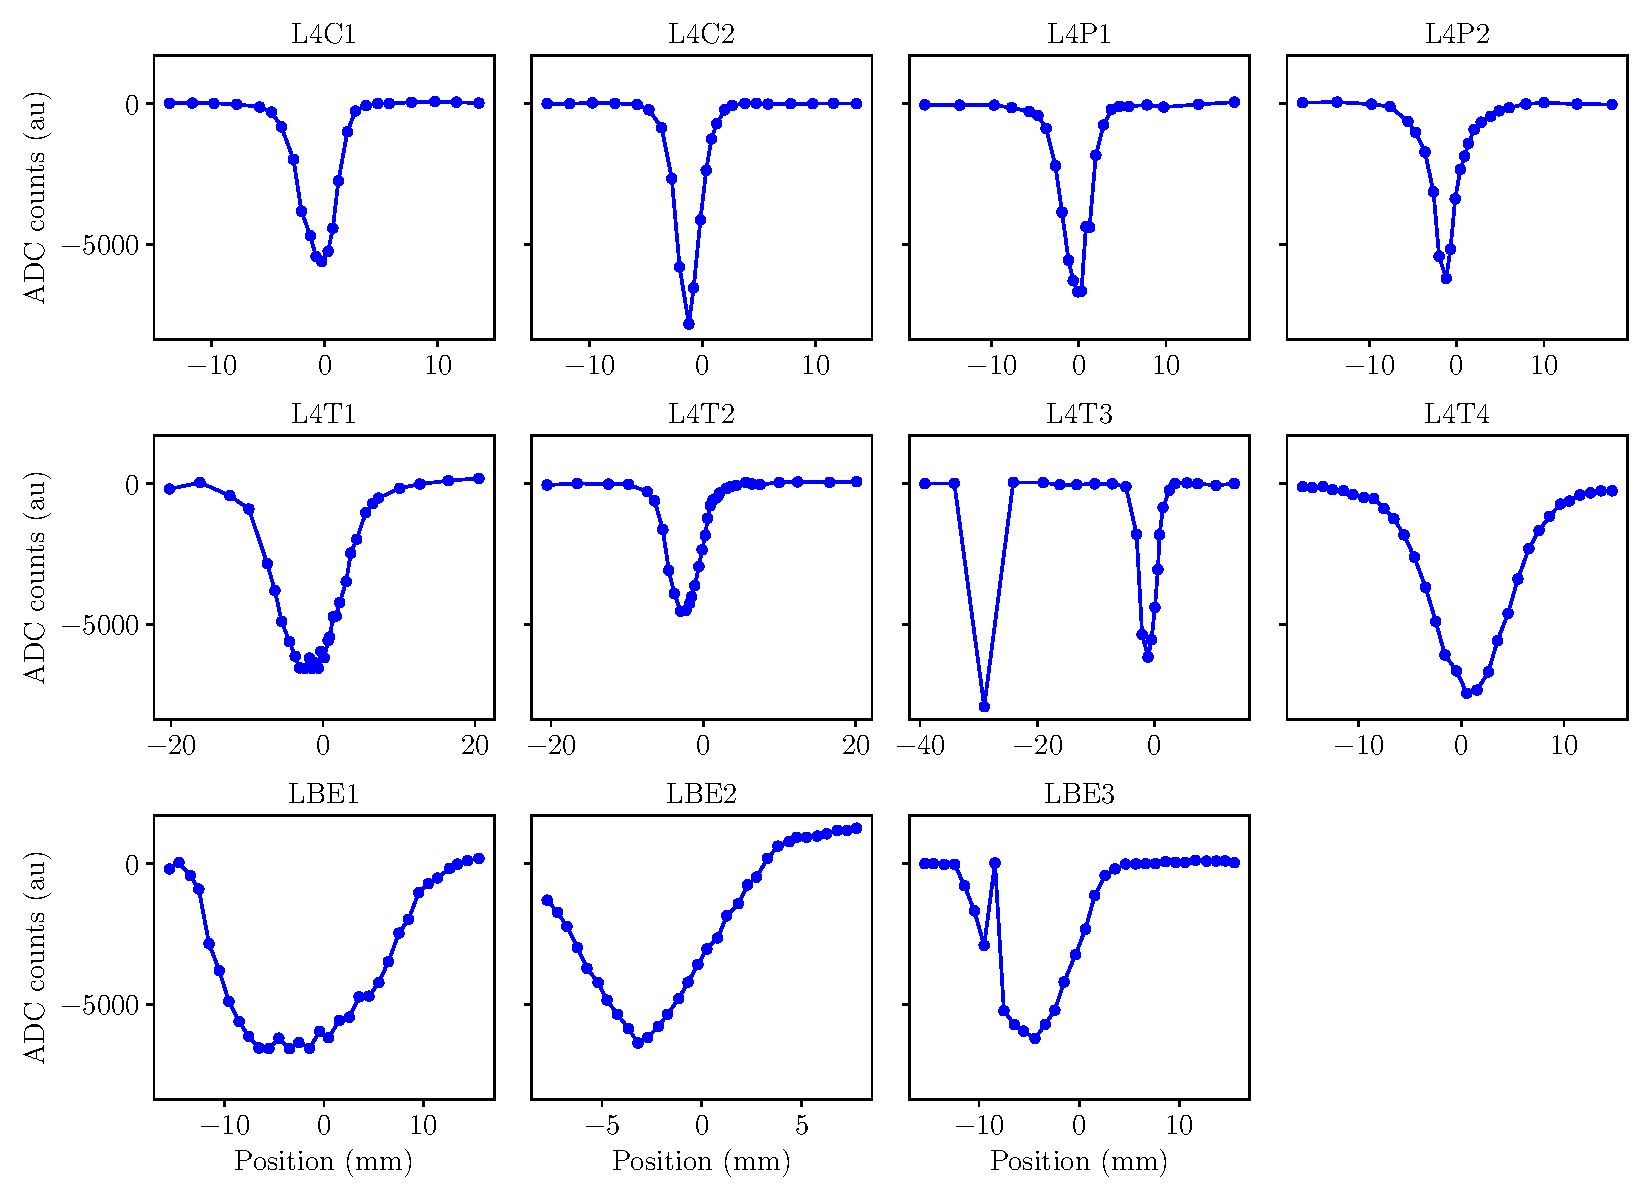
\includegraphics[width=1.0\columnwidth]{SigmaEvol/HorEvol.pdf}
    \caption{Horizontal transversal beam profile measured by the differt detectors at LINAC4}
    \label{fig:HorizontalProf}
\end{figure}

\begin{itemize}
    \item The beam profile seemed to be very much gaussian in all the measurement points except for LBE1 and LBE2 positions.
    \item Broken wires: SEM grids L4T2 and LBE3 present a broken wire that must be repaired. Wires 12-13 and 14-15 in L4P1 are glued together. 
    \item L4T1 and LBE1 present strange strange oscillations in the wires measuring the highest intensities. 
    \item Some of the grids have an even wire separation while others present a noneven wire distancing. Due to the beam not always being centered having smaller wire separation at the center of the grid des not seem to be that helpful.
    \item Not depicted, however, the data acquisition system for the detectors in the LBE sector had to be corrected to properly acquire the data.
\end{itemize}

Here we presented only the evolution of the horizontal profile, however, the evolution of the vertical profile was similarly studied. In the case of the vertical profile, a non-gaussian beam was observed in some of the locations. Figure \ref{fig:VertProf} shows an example of a vertical profile taken with both the second SEM grid and the second Wire Scanner from the L4T line. In this case, the particle beam clearly shows some shoulders or tails that push it away from the gaussian distribution. Another thing that one can observe from this figure, is the great agreement between the beam profile measurements by the sem grid and the wire scanner. 


These measurements were the first systematic set of measurements of the LBE run, they helped understand the beam evolution along the accelerator and thus helped correct the observed irregularities. These measurements also helped assess and correct any issue on the measuring devices, such as broken wires, position misreadings, data acquisition problems, etc.  

\begin{figure}[h]
    \centering
    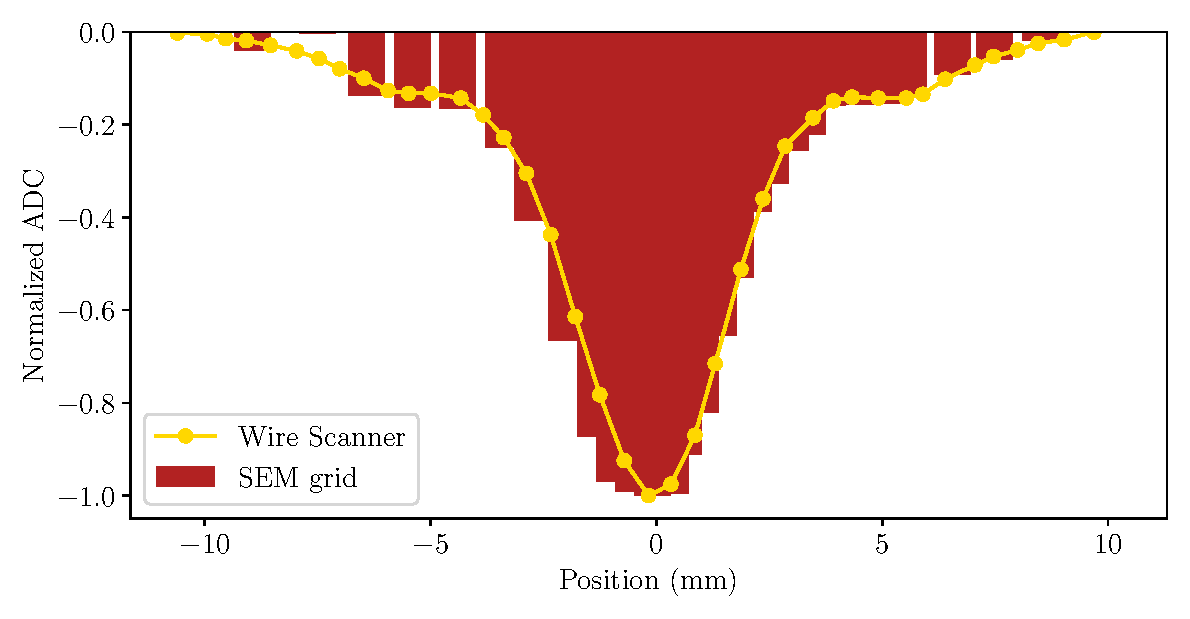
\includegraphics[width=0.6\columnwidth]{VertProf/VertProf.pdf}
    \caption{Vertical transverse profile measured by the second SEM grid and second wire scanner of the L4T line at Linac4.}
    \label{fig:VertProf}
\end{figure}

\section{Thermionic Measurements}

The best way to crosscheck the reliability of the thermal evolution simulations introduced in the previous chapter is to compare them with experimental measurements. Many techniques have been developed for measuring the temperature evolution in objects \parencite[][]{ref:ThMeas1}. 

In our particular case, we were interested in measuring experimentally the temperature evolution of thin wires ($40 \mu m$) during their interaction with the beam of particles. However, no dedicated setup could be installed in any of the CERN machines. The only information available is the intensity registered by the detectors, so we needed to find a way to obtain the detector's temperature evolution from the registered intensity.  As explained in chapter \ref{ch:CurrentModeling} among the processes contributing to the current generation we have the Thermionic emission current ($J_{th}$). This contribution to the generated current is negligible at low temperatures but it becomes considerable when higher temperatures are reached. 

The idea for these measurements was to find certain beam conditions that allowed us to reach high temperatures and thus register the thermionic current. Due to the close relationship between the thermionic current and the temperature, by comparing the simulated current and the experimentally measured one, we could judge the reliability of our thermal simulation results. 

Before starting with the experimental measurements we needed to first answer some questions: 

\subsection{Minimum detectable thermionic current}

For normal beam conditions, the currents measured by the individual wires in SEM grid, or the single wire in a Wire Scanner, are around 1 (mA). For the experimental planning, a signal was considered detectable if the thermionic current was higher than 0.05 (mA). Figure \ref{fig:ThermCurrent} shows the expected current generated in a Tungsten (40$\mu m$) and a Graphite (33 $\mu m$) wire as a function of the wire temperature. From this figure, one can observe that temperatures above 2100 (K) will be required to obtain a detectable thermionic current.  

\begin{figure}[h]
    \centering
    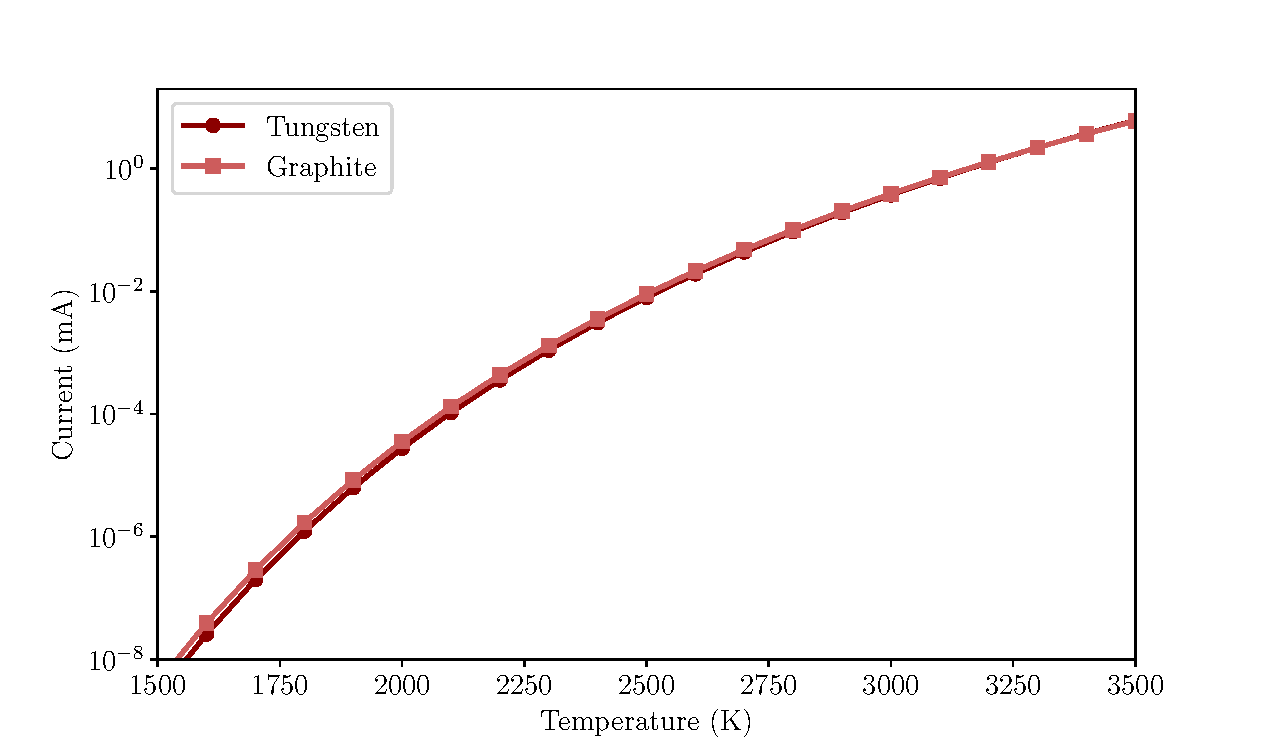
\includegraphics[width=0.80\columnwidth]{Figure_ThermoionicCurrent/ThermoCurrent.pdf}
    \caption{Thermionic current as a function of the temperature for Tungsten (40$\mu m$) and a Graphite (33 $\mu m$) wires.}
    \label{fig:ThermCurrent}
\end{figure}

\subsection{Available detectors}

Due to the high temperatures needed for performing the measurements, the risk of permanent detector damage was non-negligible. Only those detectors with already existing damage, or those placed in areas where the vacuum was intended to be disrupted could be used. 

After some deliberation, it was decided that the SEM grid L4T.BSGH/V.0243, would be used for the measurements. The beam current transformer L4T.BCT.0107 was used for continuous intensity and pulse length measurements. These detectors are located at LINAC4 in the L4T line, figure \ref{fig:DetLocation} shows the schematic representation of the location of the detector. 


\begin{figure}[h]
    \centering
    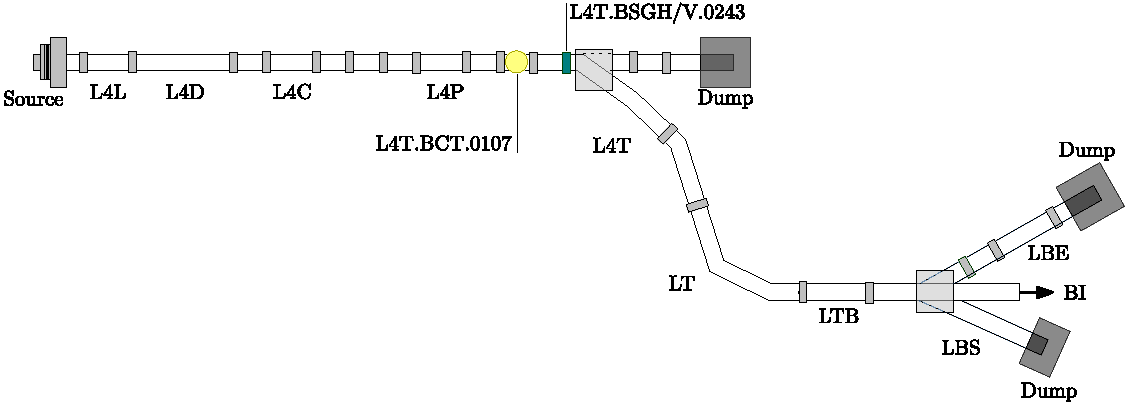
\includegraphics[width=0.90\columnwidth]{Figure_RelativePositionSemBCT/DetPosition.pdf}
    \caption{Schematic representation of Linac4 layout, with locations of the SEM Grid (L4T.BSGH/V.0243) and the BCT (L4T.BCT.0107) used for thermionic measurements.}
    \label{fig:DetLocation}
\end{figure}

The SEM grid used for the measurement was conformed of 32 Tungsten wires with gold coating. The wires had a length of 5 (cm) and a thickness of 40 $(\mu m)$. The wires were unevenly spaced, covering a total area of 40.9 (mm). Table \ref{tab:WireDist} details the locations of the different wires. The wires were placed on the top and the bottom part of the frame alternatively as shown in figure \ref{fig:WireLocation}.

\begin{table}[h]
    \centering
    \begin{tabular}{cccc}
    \hline
    Pitch              & \# of Wires & Wire Distance (mm) & Covered Region (mm) \\ \hline
    \multirow{5}{*}{3} & 6 + 6 = 12  & 0.4                & 4.4                 \\
                       & 3 + 3 = 6   & 0.75               & 8.9                 \\
                       & 3+3 = 6     & 1.0                & 14.9                \\
                       & 2 + 2 = 4   & 2.5                & 24.9                \\
                       & 2 + 2 = 4   & 4.0                & 40.9                \\ \hline
    \end{tabular}
    \label{tab:WireSpacing}
    \caption{Detailed description of wire location in SEM grid L4T.BSGH/V.0243}
\end{table}


\begin{figure}[h]
    \centering
    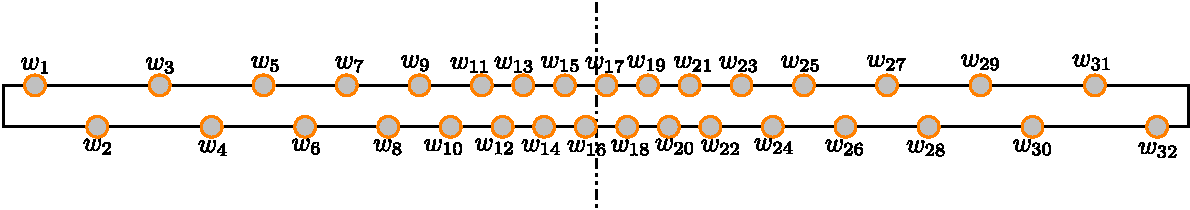
\includegraphics[width=0.90\columnwidth]{Figure_SemGridSchema/SemGridSchema.pdf}
    \caption{Schematic representation of wire position at L4T.BSGH/V.0243. }
    \label{fig:WireLocation}
\end{figure}

\subsection{Beam Conditions}

A preliminary study was performed to determine what kind of beam parameters would potentially yield a detectable thermionic current. In the L4T line, the energy of the \hm beam of particles is already 160 (MeV). The beam parameters that could be easily adjusted are: Beam intensity ($I_{beam}$), beam pulse length ($\Delta_t$), and beam size ($\sigma_x , \sigma_y$). Figure \ref{fig:Jth_Cond} shows a summary of the maximum expected thermionic current for different beam conditions. 

\begin{figure}[h]
    \centering
    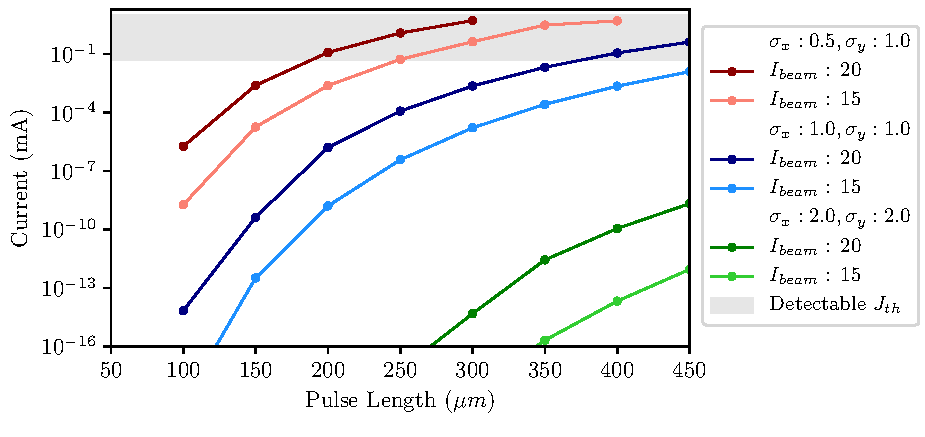
\includegraphics[width=0.90\columnwidth]{Figure_IsThereThermo/IsThereThermo.pdf}
    \caption{Summary of expected maximum current for different beam conditions. Gray Area indicates where thermionic emission is detectable. The beam size is given in (mm) and Beam intensity in (mA).}
    \label{fig:Jth_Cond}
\end{figure}

From this figure one can observe, that independently of the other beam conditions, large beam sizes ($\sigma_x = \sigma_y = 2 mm$) will not yield detectable thermionic emission. For smaller beam sizes ($\sigma_x \leq \sigma_y \leq 1 mm$), thermionic emission can be detected for long beam pulse lengths ($\Delta t > 300 \mu s$). Setting up the beam size to a specific dimension is not an easy task. Changes in the intensity of the beam also didn't produce very dramatic changes in the detectable current. During the measurements, these two quantities were kept constant while the beam pulse length was systematically increased in order to reach the thermionic stage in a controlled way. 

\section{Experimental Results}

The first set of measurements was taken using conservative beam conditions. The intensity of the beam was kept constant to $I_{beam} = 17.30 (17) mA$. Figure \ref{fig:PulseEvol} shows the evolution of the beam size during the first set of measurements. From this figure, we can see that the beam size was $\sigma_x = 1.02(5) mm$ and $\sigma_y = 1.76(2)$ mm. While the beam position remained constant around $\mu_x = -0.22(6) mm$ and $\mu_y = -0.43(21) mm$. 

\begin{figure}[h]
    \centering
    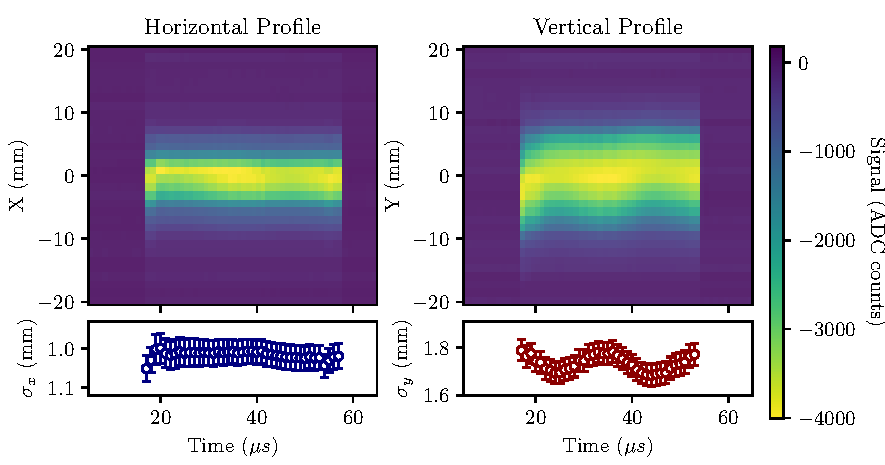
\includegraphics[width=1.0\columnwidth]{Figure_BeamProfileStudy/BeamProfEvol1.pdf}
    \caption{Evolution of the transverse beam profile along the beam pulse. Top: example of transverse beam profile measurement. Bottom: Calculated beam size from gaussian approximation. Error bars were calculated by measuring different beam pulses.  }
    \label{fig:PulseEvol}
\end{figure}

During these measurements, the beam pulse length was varied between $\Delta t = 165.38(48) \mu s$ up to $\Delta t = 247.12(33) \mu s$. As expected, no sign of thermionic emission was observed. However, when the long beam pulse lengths were measured, wires 15 and 17 were glued together. Figure \ref{fig:WireGlued} shows the current registered by the different wires as a function of time for six consecutive beam pulses. From this figure, we can see how after pulse 4, the currents registered by wires 15 and 17 are identical, indicating the wire attachment. 

\begin{figure}[h]
    \centering
    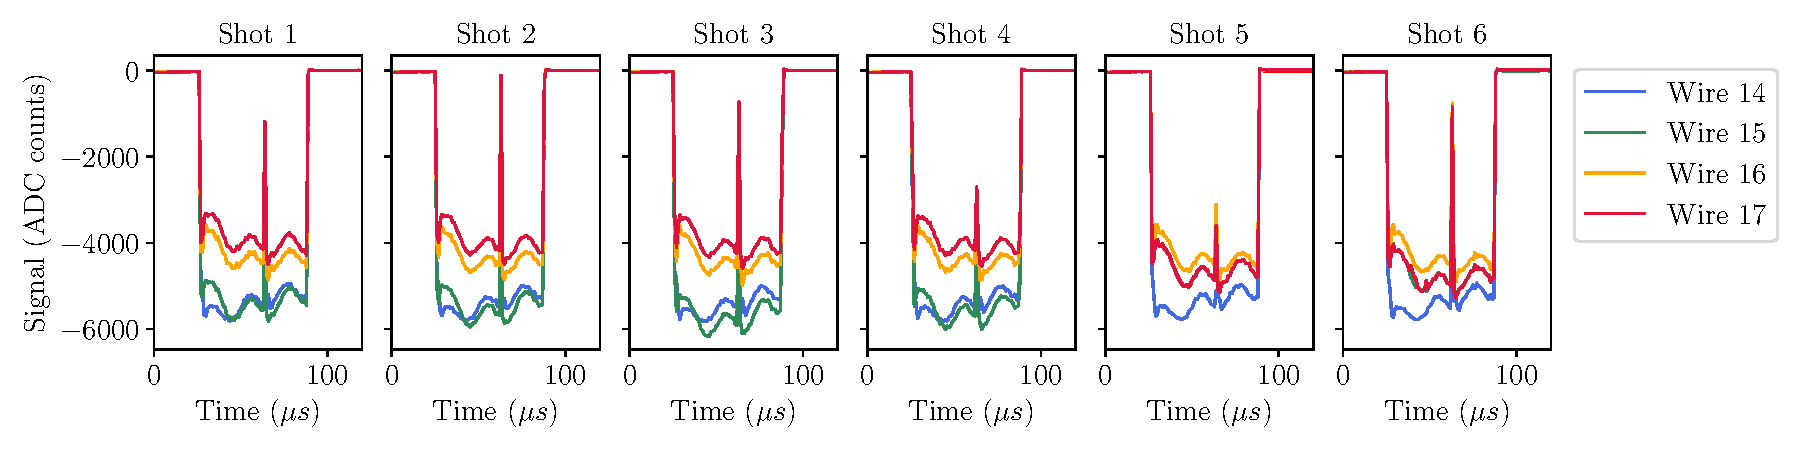
\includegraphics[width=1.0\columnwidth]{Figure_WiresGluing/WireWithTime.pdf}
    \caption{Evolution of the measured current in different wires as a function of time, for six consecutive beam pulses. }
    \label{fig:PulseEvol}
\end{figure}

In order to avoid this situation and proceed with the measurements, the beam of particles was steered away from these wires and centered around $\mu_x = -1.89(11) mm$ and $\mu_y = 1.15(31) mm$. The wire separation in this position is much larger, making wire gluing more challenging. 

To reach higher temperatures and to be able to reach the thermionic regime, the horizontal beam size was reduced to $\sigma_x = 0.59(17) mm$. As a result the vertical plane grew longer, $\sigma_y = 3.23(54) mm$. During these measurements, the beam intensity was sligtly smaller $I_{beam} \sim 16.7 mA$. The beam pulse length was increased systematically. On the vertical grid, Thermionic emission was observable in various wires for a beam pulse length of $\sim 450 \mu s$. 

\begin{figure}[h]
    \centering
    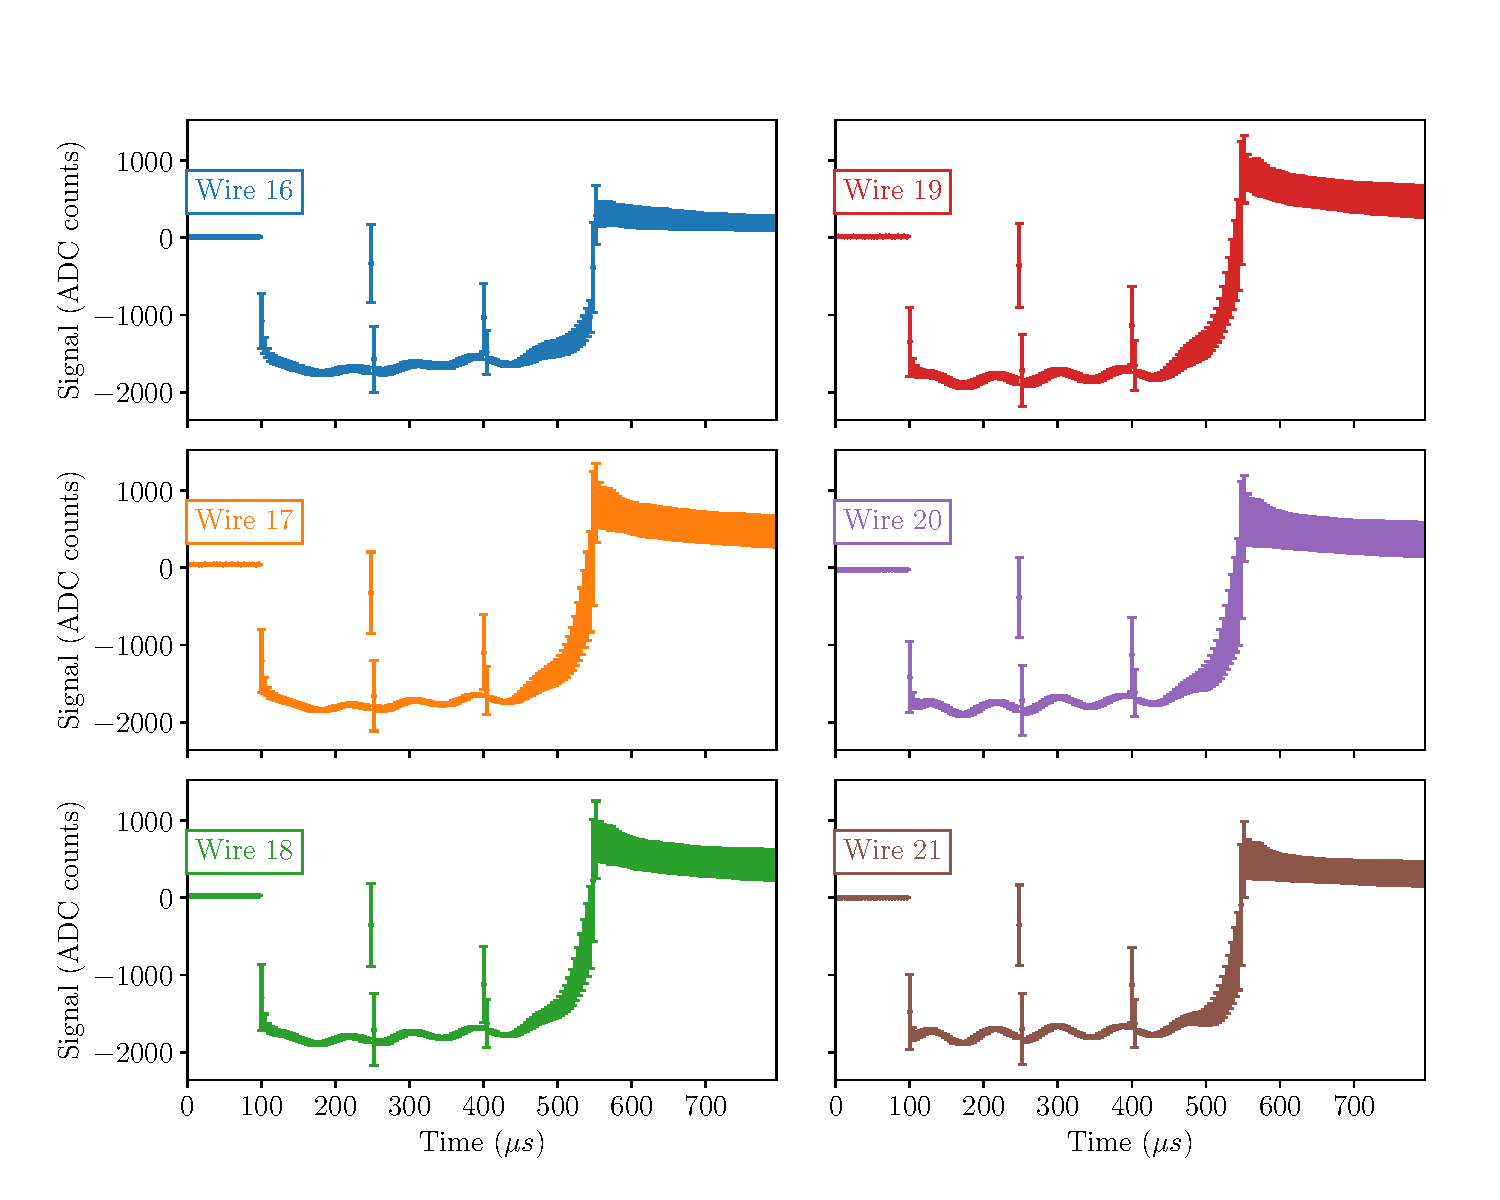
\includegraphics[width=0.9\columnwidth]{Figure_ThermionicMeasurements/VerticalThermoCurrent.pdf}
    \caption{Current registered by several wires during the beam pulse.}
    \label{fig:MeasuredThermo}
\end{figure}

Figure \ref{fig:MeasuredThermo} shows the current measured by several wires in the vertical SEM grid during the beam passage. From this figure, we can observe when the particle beam reaches the detector since a negative signal starts to be registered. As time goes by, the energy deposition in the detector material rises the temperature of the detector. As temperature increases, thermionic emission increases, and one can observe this increase in the reduction of the absolute value of the current. Once the particle beam has disappeared, a small positive current remains, because the detector is still warm, thermionic emission current is still being registered.  As the detector cools down, this current diminishes. 

In figure \ref{fig:MeasuredThermo} one can also observe some fluctuations in the registered beam current. This was an effect of the particle beam of particles itself, and could also be observed in the BCT measurements. Also, at $t = 250 \mu s$ and $t = 400 \mu s$, an anomalous value of the beam current is registered by all the wires. To avoid injection losses due to in-between rings injection, the Linac4 chopper removes part of the Linac4 beam every 150 $\mu s$. Which explains the intensity jumps registered by the wires. 

\begin{figure}[h]
    \centering
    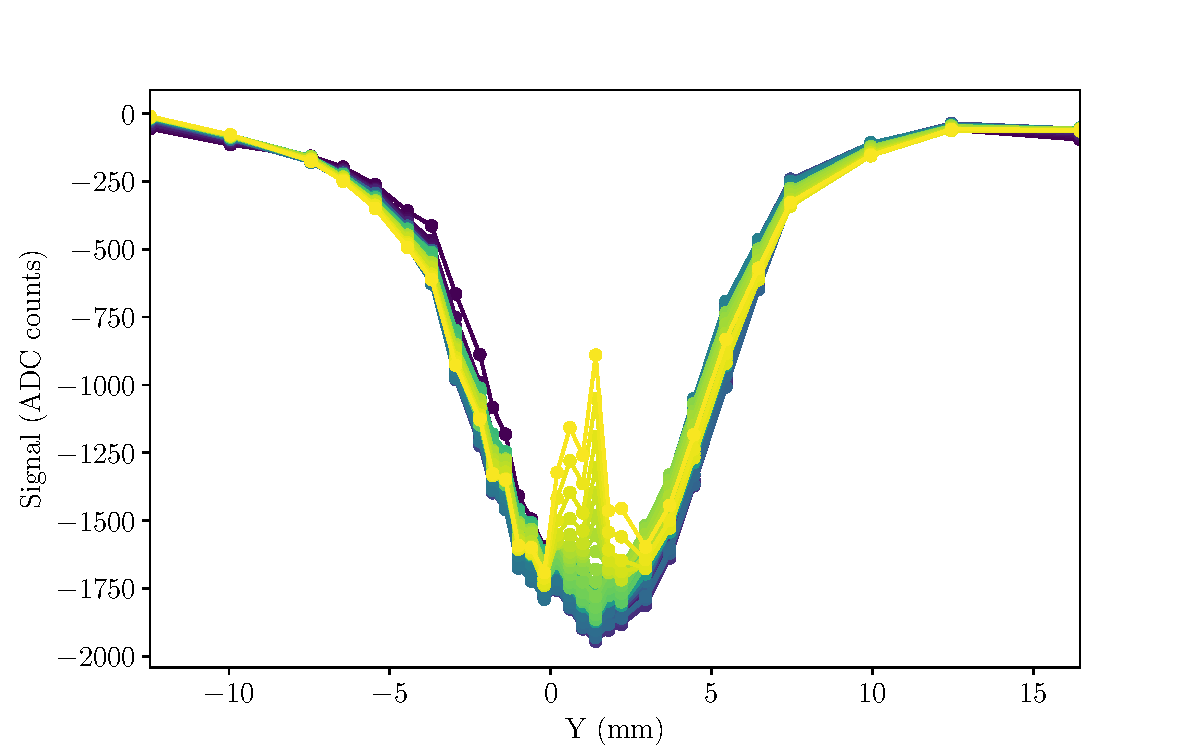
\includegraphics[width=0.75\columnwidth]{Figure_ThermionicMeasurements/ProfileJth.pdf}
    \caption{Example of vertical profile beam measurement. Darker colors indicate measurements at the beginning of the beam shot. Lighter colors indicate measurements a the end of the shot. }
    \label{fig:JthInProf}
\end{figure}

Figure \ref{fig:JthInProf} shows how thermionic emission affects the transverse beam profile measurements. In this figure, lighter currents indicate profiles taken at larger times during the beam pulse. Also from this image, we can see the absolute value of the current in the central wires diminishing as time goes by. 

\section{Measurment-Simulation Comparison}

PyTT program was used to simulate the thermal and electrical evolution of the detectors during the measurements. Figure \ref{fig:MeasSimCompa} shows a comparison between the current measured by wire 19 of the SEM grid, the simulated current, and the current measured by BCT.0107. The BCT intensity has been included in the comparison to show the intrinsic properties of the beam.

From this signal, the aforementioned beam intensity fluctuations and the chopper gaps can be also observed in the BCT measurement. However, the current reduction at longer beam pulse time is not observable in the BCT measurements, as this is an effect occurring on the wire. Also, the BCT measurement clearly shows when the beam pulse ends, proving that the positive current measured by the wire grid is not coming from the beam. 

\begin{figure}[h]
    \centering
    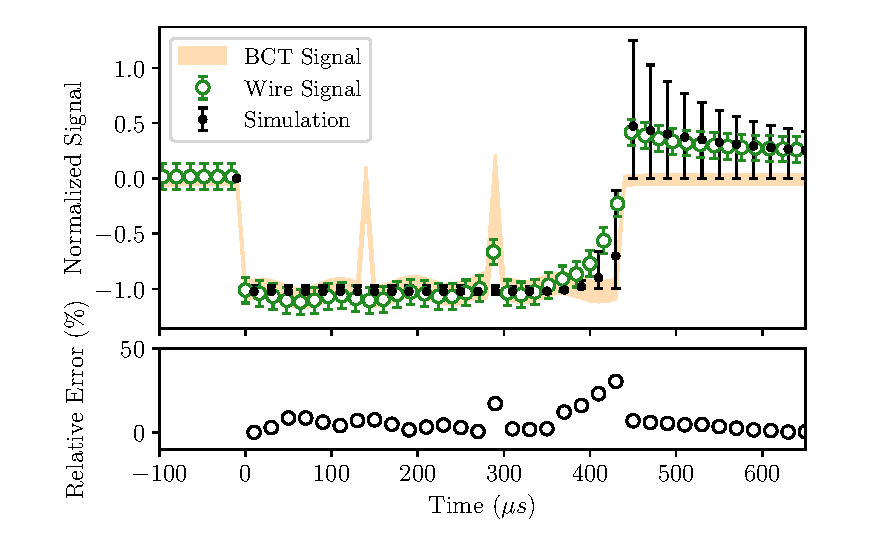
\includegraphics[width=0.75\columnwidth]{Figure_MeasurementSimulationCompa/VerticalCompa.pdf}
    \caption{Signal generated in the wire intercepting the beam as a function of time. Compared with simulated intensity results. }
    \label{fig:MeasSimCompa}
\end{figure}

Intra-pulse intensity fluctuations and chopper effects were not considered in the simulations. A constant current of $I_{beam} = 16.7 (mA)$ was considered. The simulation results seem to very clearly reproduce the average of the measured SEM current. The simulations show a slightly slower start for the thermionic emission current. However, after the beam pulse is gone, the simulated and the measured results for the thermionic current match very well. 

The maximum relative error between simulated and measured results is found to be around 30 $\%$, and it is found at the very end of the beam shot. Even then, the average relative error along the whole pulse is $6.3(25) \%$. 

A dedicated uncertainty study was performed to determine the uncertainties of the simulated results (See Section \ref{sec:ModelUnc}). In this particular case, the biggest contributor to the simulation's uncertainty came from uncertainties in the beam size. As indicated in the previous section, the beam size was $\sigma_x = 0.59(17) mm$ and $sigma_y = 3.23(54) mm$. This implies, beam size uncertainty was $\xi_x = 28.81 \%$ and $\xi_y = 16.71 \%$. As shown in section \ref{sec:ModelUnc}, uncertainties in beam sizes can yield big uncertainties in simulation results, mainly when small beam sizes are involved. 

As we saw in figure \ref{fig:MeasuredThermo}, several wires measured thermionic emission. However, due to the small changes in the measured intensity between the different wires and the big uncertainties in the simulated results, it was impossible to distinguish among them. 

\section{Simulation Comparison: Ansys}

For this work, the theory of finite differences (FDM) has been used to solve the heat equation, as was explained in Chapter \ref{ch:TempModeling}. However, FDM is just an example of numerical technique to solve PDEs and it is important to stress that alternative approaches abound. Comercially available softwares, such as Ansys \parencite[][]{ref:Ansys}, are comomnly used to accurately solve a big variety of multiphysics phenomena. In particular, Ansys uses Finite Element Analysis (FEA) \parencite[][]{ref:NumericalMethodBook} to aid the users obtain solutions for real ingeneering problems. 

The objective of this study was to compare the results obtained with the PyTT code, with results obtained with Ansys, a highly used and benchmarked comercially available software. 

\subsection{Thin Wire Studies}

The first part of this study compares the thermal evolution results, of a thin tungsten wire ($\phi$ = 40 $\mu m$), calculated with the PyTT code and Ansys. Here, a LINAC4-like beam of particles was considered as the heating source. Table \ref{tab:BeamParametersCompa} summarizes the parameters of the beam. The parameters on this table remained constant for all the simulations. The beam pulse length was systematically varied in order to cover differnt temperature ranges. 

\begin{table}[h]
    \centering
    \begin{tabular}{ccccc}
    \hline
    Particle & \begin{tabular}[c]{@{}c@{}}Energy\\ (MeV)\end{tabular} & \begin{tabular}[c]{@{}c@{}}Inensity\\ (mA)\end{tabular} & \begin{tabular}[c]{@{}c@{}}Sigma x \\ (mm)\end{tabular} & \begin{tabular}[c]{@{}c@{}}Sigma y\\ (mm)\end{tabular} \\ \hline
    Proton   & 160   & 25      & 0.5           & 1.                        \\ \hline
    \end{tabular}
    \caption{Summary of the beam parameters that remained constant during the simulations.}
    \label{tab:BeamParametersCompa}
\end{table}

To achieve the closes simulation conditions, a cuboid approximation of the wire was considered in both, PyTT and Ansys. The wire was oriented along the y axis, with a wire lenght of 2 (cm). The spatial mesh resolution was of 0.1 (cm) along the wire lenght and for the x and z directions a single mesh element was considered. The temporal resolution was divided in two sections. During the beam pulse, temporal elements of $10^{-7}$ (s) where considered, while during the cooling section the temporal elements were $10^{-4}$ (s) long. Material parameters, such as heat capacity and conductivity, were considered to be temperature dependent. However the emissivity was considered to be constant and equal to 0.1 in both cases. 

\begin{figure}[h]
    \centering
    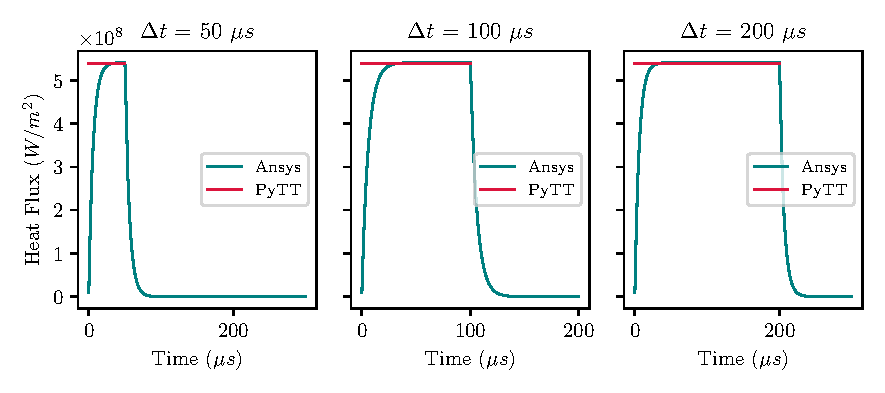
\includegraphics[width=1.0\columnwidth]{HeatInpuCompa/HeatInputCompa.pdf}
    \caption{Examples of the heat flux provided to Ansys and PyTT for three different simulation cases.}
    \label{fig:AppliedHeatWire}
\end{figure}

In Ansys, the heat load was given using APDL commands \parencite[][]{ref:APDLCommand}. Here, a gaussian distribution with the heat flux ($W/m^2$) equvalent of a beam pulse was described and applied to the material surface. Figure \ref{fig:AppliedHeatWire} shows the heat flux applied to the wire by both Ansys and PyTT. The heat load in PyTT is constant during the presence of the beam pulse, and it inmediately goes to zero oncethe beam pulse has passed. In the case of Ansys, a more smooth heat load transition is observed. The total integrated heat flux was the same in both programs, with a maximum discrepancy of $0.64\%$ for the shorter beam pulses ($\Delta t \leq 50\mu s$). 

Figure \ref{fig:TemperatureComparison} compares evolution of the maximum temperature, for three different beam pulse lengths, as a function of time. In this figures, one can obser how the PyTT simulations systematically give a higher maximum temperature than the results obtained with Ansys. Nonetheless, the cooling rate is the same in both cases. The maximum discrepancy between the Ansys and the PyTT resulsts was of $11.2\%$ for a temperature of 1356K.

\begin{figure}[h]
    \centering
    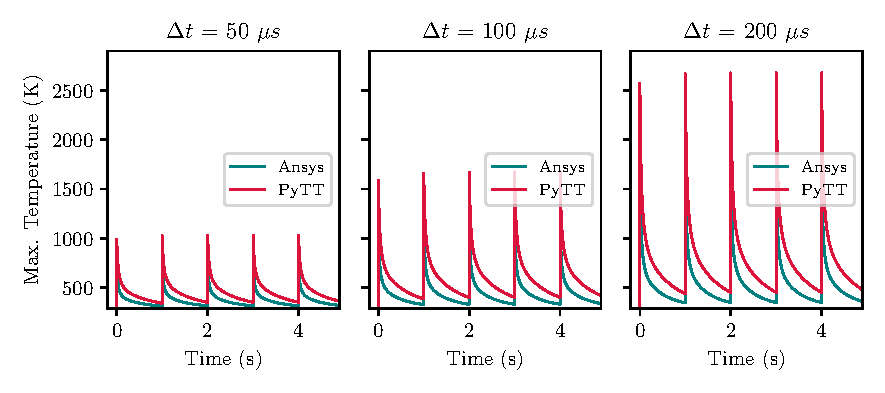
\includegraphics[width=1.0\columnwidth]{TempCompa/TempCompa.pdf}
    \caption{Comparison of the evolution of the maximum temperature in the detector as a function of time, for three different beam pulse lengths.}
    \label{fig:TemperatureComparison}
\end{figure}

One big difference between this two programs when performing this study was the simulation time. PyTT averaged 10.56 (s) when performing these simulations, while Ansys averaged 7:35 (min), in an Hp Intel(R) Core(TM) i7-6700 CPU, 16.0 Go RAM. This comparison might not be totally fair, Ansys is a much more complex simulation tool, with many many more options and accurate models. With the appropiate knowledge, the simulation times can be optimized. However, if what it is important is to quicly obtain a number that can give the user if certain beam parameters are going to damage or not a detector, the PyTT code can manage to do it fast, with results that are very similars to the ones obtained with Ansys. 

\subsection{Thin Foil Studies}

Similar Studies were performed with thin graphite foils ( dimensions = 2 (cm) x 2 (cm) x 40 ($\mu m$)). The beam conditions for this studies were the same as the ones described in table \ref{tab:BeamParametersCompa}. Variations on the beam pulse lenght were used again to control the maximum temperature reached by the detectos. Figure \ref{fig:TempMaxErrCompa} shows the maximum temperature reached (at equilibrium), with both PyTT and Ansys codes, as a function of the beam pulse length. From this figure one can see how at higher temperatures PyTT continues systematically giving a higher maximum temperature. However, at lower temperatures, ansys gives higher maximum temperature results. The relative error between the ansys and PyTT results is higher at lower beam pulse lengths, however it never exceeds a $20 \%$.

\begin{figure}[h]
    \centering
    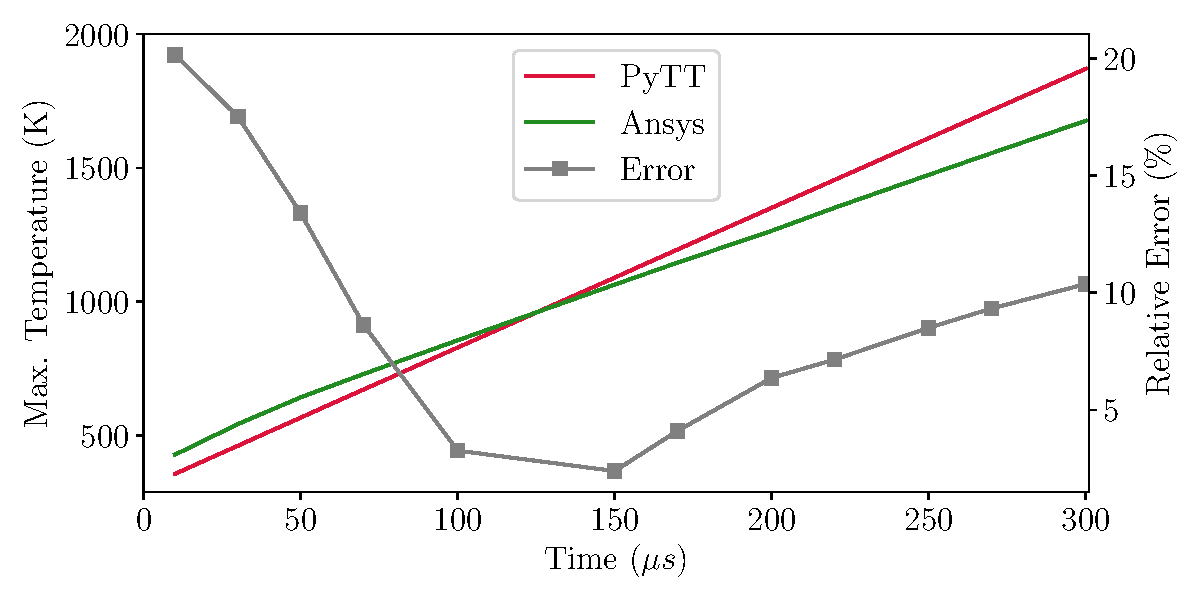
\includegraphics[width=0.6\columnwidth]{ErrorCompa/FoilMaxTempCompa.pdf}
    \caption{Comparison of the evolution of the maximum temperature in $40 \mu m$ graphite foil, as function of beam pulse lenght. On the right axis, the relative error between is represented. }
    \label{fig:TempMaxErrCompa} 
\end{figure}

\begin{figure}[h]
    \centering
    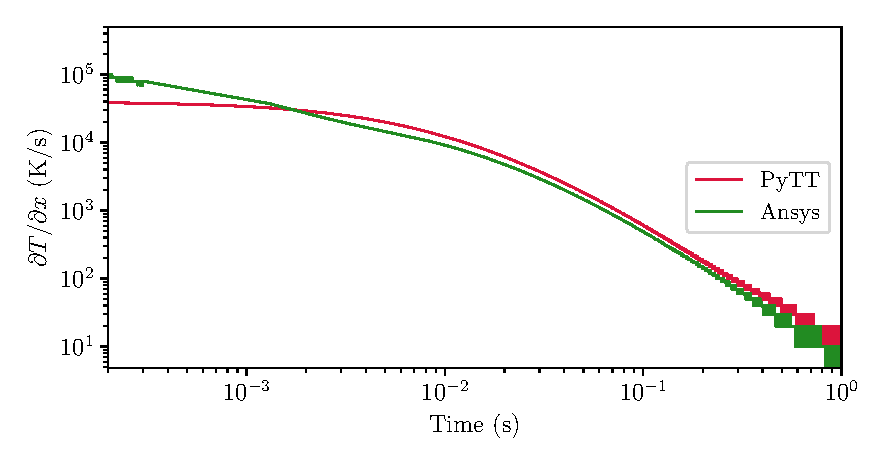
\includegraphics[width=0.6\columnwidth]{CoolingSpeedAnsys/CoolingSpeed.pdf}
    \caption{Comparison of the cooling rate between PyTT code and Ansys. For a $40 \mu m$ graphite foil after a beam shot. }
    \label{fig:CoolingRate} 
\end{figure}

For a beam pulse lenght of $100 (\mu s)$, the cooling rate was calculated with Ansys and with PyTT. Figure \ref{fig:CoolingRate} shows a comparison between the cooling rate after a beam shot. From this figure we can observe how Ansys presented a much faster cooling at the beggining (higher temeperatures) and a slower cooling after some time (lower temperatures). Here, the temperature right after the beam shot was 848 (K).

Another interesting feature we wanted to compare was the heat distribution in space. Figure \ref{fig:FancyPlotComparison} shows the heat distribution of the foil simulated with Ansys (left) and the PyTT code (right). This two figures ware taken at the same instant of time (10 ms), during the cooling process. It is clear from this pictures that the heat distribution is  very similar in both cases. Because the heating in Ansys is faster, at the same instant of time, the maximum temperature reported is smaller. 

It is very difficult to properly understand the differences between these results. Information about the numerical methods employed by ansys is not publically available. So no more quantitative or in depth conclusions could be taken from these studies. 

\begin{figure}[h]
    \centering
    \begin{subfigure}[b]{0.45\textwidth}
        \centering
        \includegraphics[width=\textwidth]{AnsysPyTT_2Dcompa/Ansys2DPlot.png}
    \end{subfigure}
    \hfill
    \begin{subfigure}[b]{0.5\textwidth}
        \centering
        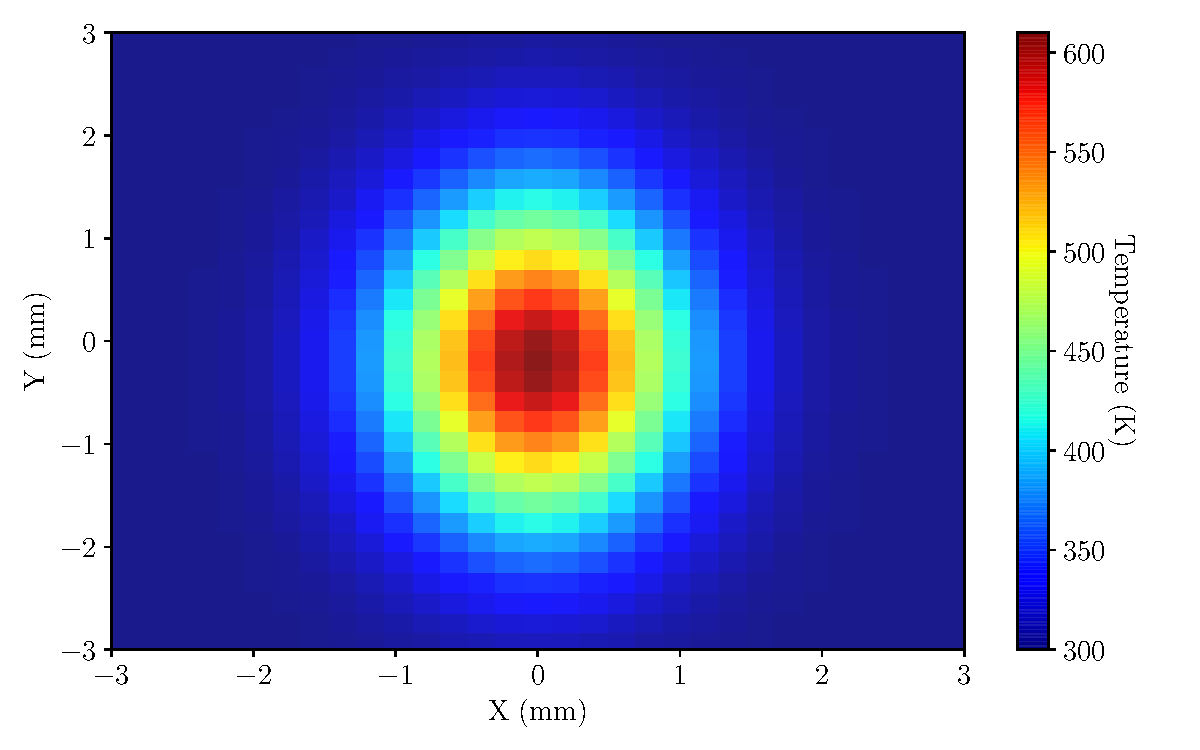
\includegraphics[width=\textwidth]{AnsysPyTT_2Dcompa/FoilPyTT.pdf}        
    \end{subfigure}

    \caption{Comparison between thermal distribution in Graphite foil affter one beam shot. In ansys (left) and PyTT code (Right). The black lines in ansys have a separation of 1 (mm).}

    \label{fig:FancyPlotComparison} 
\end{figure}


\section{Aplications: Beam Power Limit Calculations}

Determining beam power limits means determining beam conditions that could potentially damage the detectors. To do that, the PyTT program was used to simulate the maximum temperatures reached by the detectors for the different expected beam conditions at their location. If the maximum temperature reached was above the safe limit, those beam conditions were considered to be harmful to the detectors. 

\subsection{SEM grid and Slow Wire Stanner at Linac4}

For Linac4, the beam conditions under study were: Beam Intensity ($I_{beam}$), beam pulse length ($\Delta t$) and beam size ($\sigma_x , \sigma_y$). Figure \ref{fig:DetLoc} shows a schematic representation of Linac4, with the different detectors location. The detectors in the L4L, L4D and L4C lines are made of graphite wires ($33 \mu m$). The rest of the wire scanner detectors are also graphite wires, whereas the SEM grid detectors are gold-coated tungsten wires ($40 \mu m$). Table \ref{tab:beamprop} summarizes the range of the beam properties expected at the Linac4 accelerator.

For each detector, a set of dedicated simulations covering the whole parameter range were performed with the PyTT program. A maximum temperature of 1400K was taken as a safe maximum temperature limit. This limit is probably very conservative, as most of the detectors could easily handle up to 3000 K. However, due to the wire-gluing problem suffered in SEM grid detectors, a much lower temperature limit was established. 

\begin{figure}[h]
    \centering
    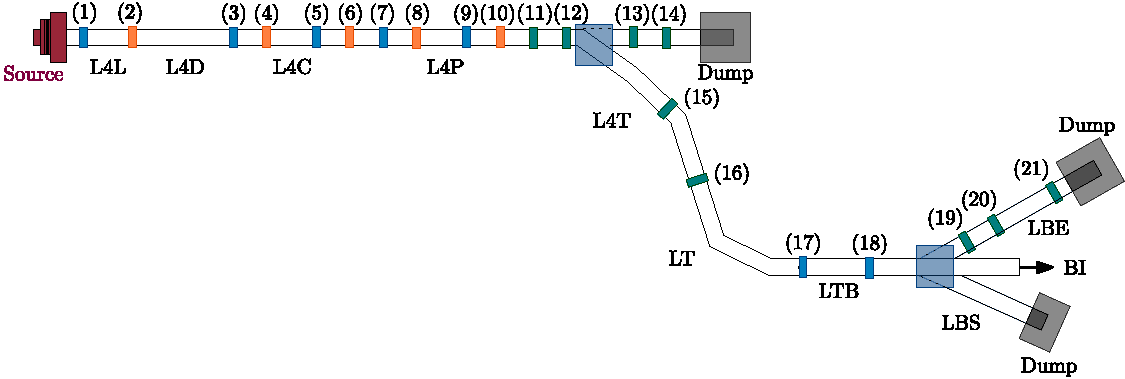
\includegraphics[width=1.0\columnwidth]{Figure_Linac4Instrumetnation/DetecPos.pdf}
    \caption{Schematic representation of Linac4 with SEM grid (blue boxes), wire scanner (orange boxes) locations. Green boxes indicate locations where both, sem grid and wire scanners are installed.}
    \label{fig:DetLoc}
\end{figure}


\begin{table}[h]
    \centering
    \begin{tabular}{cccc}
    \hline
    Property                          & Min & Max & Units   \\ \hline
    Intensity ($I_{beam}$)            & 10  & 25  & mA      \\
    Pulse Length ($\Delta t$)         & 50  & 400 & $\mu s$ \\
    Beam Size ($\sigma_x , \sigma_y$) & 0.5 & 3.0 & mm      \\ \hline
    \end{tabular}
    \caption{Range of beam properties expected at Linac4 accelerator.}
    \label{tab:beamprop}
\end{table}

Figure \ref{fig:EnerCompa} shows an example of the power limits calculated for a detector in L4C line (Detector 5) and a detector at the L4T line (Detector 12). Each square represents the maximum temperature reached by a simulation with the beam pulse length indicated on the X axis, and the beam intensity indicated on the Y axis. The beam size in both cases was $\sigma_x = \sigma_y = 2.0 (mm)$ . 

In both cases, we can observe that beam pulse lengths smaller than 200 $\mu s$ are very safe. Neither detector was getting close to the set temperature limit. One interesting observation is in this case the difference in the results between the detector located at the L4C line and the one located at the L4T line. The only difference between the detectors is the energy deposition in the material. At higher energies, the energy deposition is smaller, so the maximum temperatures reached by the detector are smaller than the equivalent conditions at lower energies. 

\begin{figure}[h]
    \centering
    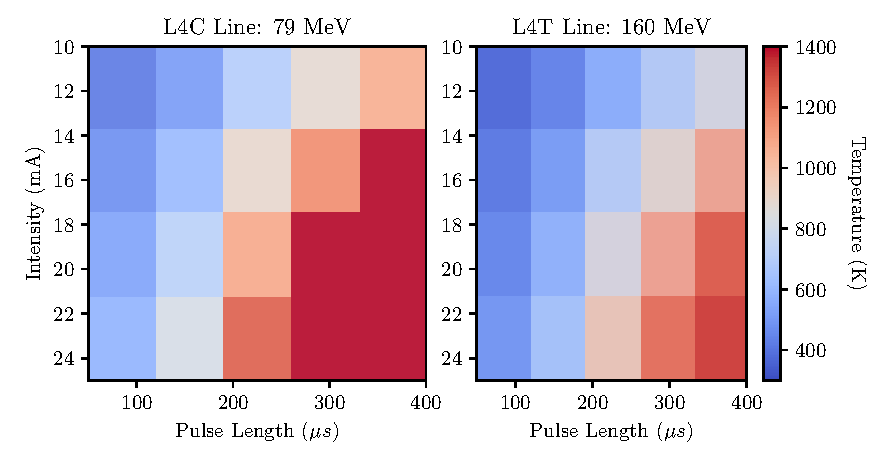
\includegraphics[width=1.0\columnwidth]{Figure_ThermalLimitsSquares/EnergyCompa.pdf}
    \caption{Power limit calculations for a detector at L4C (Left) and a detector at L4T (right) lines. The beam size in both cases was $\sigma_x = \sigma_y = 2.0 (mm)$.}
    \label{fig:EnerCompa}
\end{figure}

Figure \ref{fig:SigmaComparison} shows a similar set of results, but this time, both detectors were placed at locations where the particle energy was already 160 MeV. The difference between the right plot and the left plot is the beam size. The left hand side figure pictures a small beam size ($\sigma_x = 0.8$ (mm), $\sigma_y = 2.0$ (mm)). The right-hand side figure pictures a larger beam size ($\sigma_x = 1.2 (mm)$). From this figure, we can observe how small beam sizes result in much more critical thermal conditions. 

In general, one should be very careful measuring small beam sizes at low energy ranges. An overall power limit for the Linac4 accelerator was established. Beam conditions were considered to be dangerous if the beam size was smaller than 1 $(mm)$ and the beam pulse length was longer than $100 ()\mu s)$. An interlock system for SEM grids and wire scanners was established at Linac4 based on these results. 

\begin{figure}[h]
    \centering
    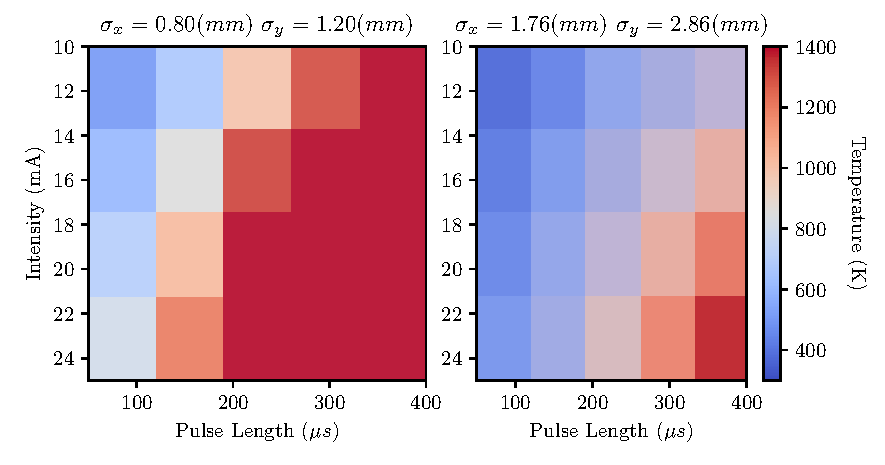
\includegraphics[width=1.0\columnwidth]{Figure_ThermalLimitsSquares/SigmaCompa.pdf}
    \caption{Power limit calculations for a detector at 160 MeV beam energies.}
    \label{fig:SigmaComparison}
\end{figure}

\subsection{Fast Wire Scanners at SPS}

A new generation of beam wire scanners has been developed at CERN, in the framework of the LIU project \parencite[][]{ref:WireScanJose}. In the SPS, 4 new wire scanner systems were installed, for horizontal and vertical beam size measurements. In this case, the relevant parameters under study were: beam emittance (at injection and extraction), the number of protons per bunch (from $10^9$ to $10^{11}$), the maximum number of bunches (from 1 to 288) and wire scanner velocity (form 1 m/s to 20 m/s). 

For the SPS energies ( 26 GeV at injection and 450 GeV at extraction ) differences in energy deposition are not as important as in the Linac4 case. Beam sizes are still a very important parameter to consider. In the SPS, the beam size is usually described in terms of beam emittance. One can easily convert from one to the other with the following relation: 

\begin{equation}
    \sigma = \sqrt{\frac{\epsilon_{norm}}{\gamma_{rel} \cdot \beta_{rel}} \cdot \beta(s)}
\end{equation}

Where $\epsilon_{norm}$ refers to the normalized emittance and $\beta_{rel}$, $\gamma_{rel}$ are the relativistic parameters. $\beta(s)$ is the courant-Snyder parameter at the position s. Because the beam size decreases as the relativistic parameters increase, smaller beam sizes are found in the extraction case. 

Figure \ref{fig:WireScanner1} shows the evolution of the maximum temperature reached by a 33 $\mu m$, graphite, fast wire scanner for a different number of particles per bunch. In this figure, the wire scanner speed was set constant to 1 m/s, and the total number of bunches was always 288.  The figure on the left is for injection energies (26 MeV) and the one on the right is for extraction energies (450 MeV). In both cases, the higher the number of particles per pulse the higher the temperature reached by the detector. 

In these figures, we can also see the decrease of the beam size with the energy, as the temperature increase happens in a much narrower period during extraction energies. 

\begin{figure}[h]
    \centering
    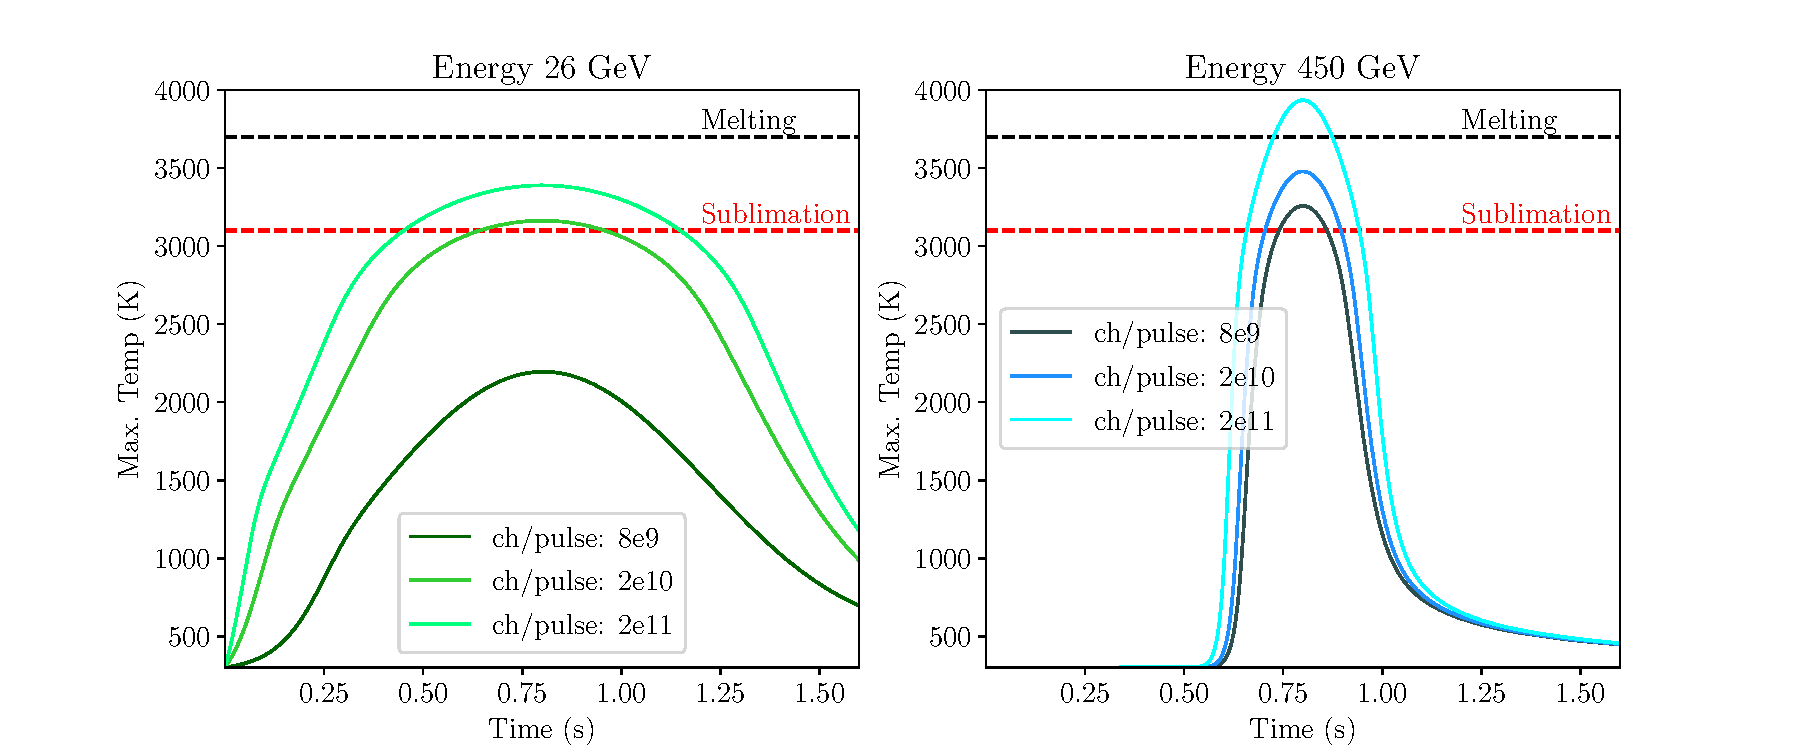
\includegraphics[width=1.0\columnwidth]{WireScanner_Limits/WireLim1.pdf}
    \caption{Comparison of maximum fast wire scanner temperatures reached for different beam conditions. Left: Injection energy. Right: Extraction energy.}
    \label{fig:WireScanner1}
\end{figure}

The wire velocity is also a very important factor to consider. The slower the wire velocity the longer time it will spend in the central area of the beam, and thus the higher the maximum temperature reached. Increasing the wire speed is beneficial in terms of thermal limitations. However, as a tradeoff, we have the measurement resolution. Because the wire scanner in the SPS is much slower than the bunches being accelerated (revolution period $t_{rev} = 2.4\cdot 10^{-5} s$). The number of points per sigma taken by a fast wire scanner can be calculated as: 

\begin{equation}
    n_{points} = \frac{\sigma}{v_{w}\cdot T_{rev}}
\end{equation}

For a beam size of 1 mm, a maximum speed of 10 m/s can be used. Otherwise, the measurements would not have enough resolution. 

The wire damage can be associated with the density of charges traversing the wire \parencite[][]{ref:Msapinski}:

\begin{equation}
     n_{ch} = \frac{N_{ch} \cdot d_{w}}{v_{w} \cdot t_{rev} \cdot \sigma}
\end{equation}

Where $N_{ch}$ is the total number of particles, understood as the number of particles per pulse times the number of pulses. $d_w$ is the wire diameter and $v_w$ is the wire velocity. As a limiting scenario, we could consider the case of a 33 $\mu m$ Graphite wire, with a speed of 1 m/x and measuring a beam size $\sigma_x = \sigma_y = 0.3$ (mm).   In this case the density of particles $n_{ch} = 2.5\cdot 10^{12}$. Beam and wire conditions yielding a charge density higher than this number, are considered to be potentially harmful.

This number is consistent with the experiments performed by M. Sapnski \parencite[][]{ref:Msapinski}. This value is used in the SPS accelerator as a safety limit. Table \ref{tab:MaxNturns} shows an example of how this safety value was used to calculate the maximum number of allowed turns for different wire scanners and beam conditions. At CERN SPS, the maximum number of injected turns can go up to 288. From this table, we can observe that only at injection energies this number of bunches can be measured. 

% Please add the following required packages to your document preamble:
% \usepackage{multirow}
\begin{table}[h]
    \centering
    \begin{tabular}{cclccccc}
    \hline
    \multirow{2}{*}{\begin{tabular}[c]{@{}c@{}}Energy \\ (GeV)\end{tabular}} & \multicolumn{2}{c}{Beam Size (mm)} & \multicolumn{5}{c}{Wire Velocity (m/s)} \\ \cline{2-8}    & $\sigma_x$               & $\sigma_y$              & 1     & 6      & 10    & 15    & 20     \\ \hline
    \multirow{2}{*}{25}                                                      & 3.03             & 2.10            & 54    & 323    & 538   & 807   & 1080   \\
     & 2.0              & 1.38            & 35    & 213    & 350   & 531   & 708    \\ \hline
    \multirow{2}{*}{450}   & 0.72             & 0.50            & 12    & 74     & 129   & 194   & 258    \\    & 0.47             & 0.33            & 8     & 51     & 85    & 127   & 170    \\ \hline
    \end{tabular}
    \caption{Maximum allowed number of beam bunches for different beam conditions. The number of charges per bunch was $1.5 \cdot 10^{11}$ ch/bunch. }
    \label{tab:MaxNturns}
\end{table}

